\documentclass[11pt]{beamer}
\usetheme{Madrid}
\usefonttheme{serif}

\usepackage[english]{babel}
\usepackage{amsmath,amssymb,mathtools}
\usepackage{tikz}
\usetikzlibrary{arrows.meta,positioning,calc}

\definecolor{accent}{RGB}{55,55,180}
\definecolor{diagramblue}{RGB}{48,103,166}
\definecolor{diagramred}{RGB}{178,65,56}
\definecolor{diagramgreen}{RGB}{47,128,92}
\definecolor{softgray}{RGB}{118,118,118}
\definecolor{lightgray}{RGB}{224,224,224}

\setbeamercolor{structure}{fg=accent}
\setbeamercolor{frametitle}{fg=white,bg=accent}
\setbeamercolor{title}{fg=white,bg=accent}
\setbeamercolor{palette primary}{fg=white,bg=accent}
\setbeamercolor{palette secondary}{fg=white,bg=accent!88!black}
\setbeamercolor{palette tertiary}{fg=white,bg=accent!74!black}
\setbeamercolor{palette quaternary}{fg=white,bg=accent!62!black}
\setbeamercolor{normal text}{fg=black,bg=white}
\setbeamertemplate{navigation symbols}{}
\setbeamersize{text margin left=0.68cm,text margin right=0.68cm}

\newcommand{\eyebrow}[1]{%
  {\color{accent}\bfseries #1}\par
  \vspace{0.04cm}{\color{lightgray}\rule{\linewidth}{0.45pt}}\vspace{0.10cm}}
\newcommand{\keyterm}[1]{\textcolor{accent}{\bfseries #1}}
\newcommand{\dd}{\,\mathrm d}

\title[Algebraic \& Dynamics on Networks]{Algebraic and Stochastic Dynamics on Directed Networks}
\author[H. Zhang]{Heze Zhang}
\date{October 7, 2026}

\begin{document}

% 1
\begin{frame}
  \titlepage
\end{frame}

% 2
%=======================================================================================================================
\begin{frame}{Agenda}
  \vspace{0.35cm}
  \tableofcontents[hideallsubsections]

  \vfill
  {\small\color{softgray}
  From a Boolean encoding of directed graphs to stochastic evolution of structural observables.}
  \vspace{0.35cm}
\end{frame}
%=======================================================================================================================

%%%%%%%%%%%%%%%%%%%%%%%%%%%%%%%%%%%%%%%%%%%%%%%%%%%%%%%%%%%%%%%%%%%%%%%%%%%%%%%%%%%%%%%%%%%%%%%%%%%%%%%%%%%%%%%%%%%%%%%%
\section{Algebraic Framework}

% 3
\begin{frame}{One Coherent Mathematical Architecture}
  \small
  \eyebrow{The organizing principle}

  \begin{center}
  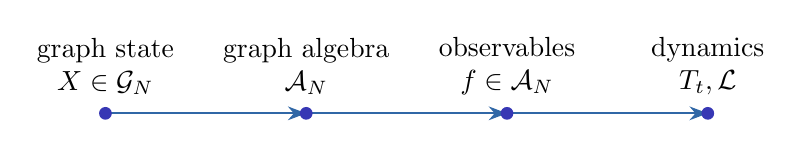
\begin{tikzpicture}[>=Stealth,thick,x=1cm,y=1cm]
    \coordinate (a) at (0.6,0);
    \coordinate (b) at (3.15,0);
    \coordinate (c) at (5.70,0);
    \coordinate (d) at (8.25,0);
    \draw[->,diagramblue] (a) -- (b);
    \draw[->,diagramblue] (b) -- (c);
    \draw[->,diagramblue] (c) -- (d);
    \foreach \p in {a,b,c,d}{\fill[accent] (\p) circle (2.3pt);}
    \node[align=center,above=3pt] at (a) {graph state\\$X\in\mathcal G_N$};
    \node[align=center,above=3pt] at (b) {graph algebra\\$\mathcal A_N$};
    \node[align=center,above=3pt] at (c) {observables\\$f\in\mathcal A_N$};
    \node[align=center,above=3pt] at (d) {dynamics\\$T_t,\mathcal L$};
  \end{tikzpicture}
  \end{center}

  \vspace{0.55cm}
  \begin{columns}[T,onlytextwidth]
    \begin{column}{0.48\textwidth}
      \keyterm{Algebraic layer}\par
      Edge variables generate a finite-dimensional commutative algebra that represents every function on the graph state 
      space.

      \vspace{0.35cm}
      \keyterm{Structural layer}\par
      Relabeling-invariant elements encode motifs and macroscopic network statistics.
    \end{column}
    \begin{column}{0.48\textwidth}
      \keyterm{Probabilistic layer}\par
      A continuous-time Markov process specifies random transitions between graph states.

      \vspace{0.35cm}
      \keyterm{Dynamical layer}\par
      The generator turns microscopic transition rules into evolution equations for observables.
    \end{column}
  \end{columns}
\end{frame}

% 4
\begin{frame}{Microscopic State Space}
  \small
  \begin{columns}[T,onlytextwidth]
    \begin{column}{0.61\textwidth}
      \eyebrow{Directed graphs as Boolean configurations}
      \begin{align*}
        V_N &= \{1,\ldots,N\},\\
        \overrightarrow{\mathcal E}_N
        &= \{(i,j)\in V_N^2:i\neq j\},\\
        \mathcal G_N
        &= \{(V_N,E):E\subseteq\overrightarrow{\mathcal E}_N\}.
      \end{align*}
      For $X\in\mathcal G_N$, define one indicator per possible edge:
      \[
        x_{ij}(X)=\mathbf 1_{\{(i,j)\in E(X)\}}.
      \]
      Hence
      \[
        \mathcal G_N\cong\{0,1\}^{N(N-1)},
        \qquad |\mathcal G_N|=2^{N(N-1)}.
      \]
    \end{column}
    \begin{column}{0.34\textwidth}
      \centering
      \vspace{0.65cm}
      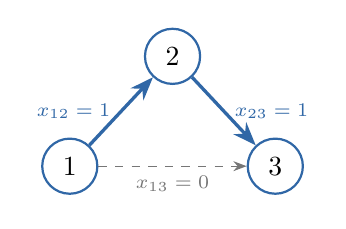
\begin{tikzpicture}[>=Stealth,scale=0.90]
        \node[circle,draw=diagramblue,thick,minimum size=7mm] (n1) at (0,0) {$1$};
        \node[circle,draw=diagramblue,thick,minimum size=7mm] (n2) at (1.45,1.55) {$2$};
        \node[circle,draw=diagramblue,thick,minimum size=7mm] (n3) at (2.9,0) {$3$};
        \draw[->,very thick,diagramblue] (n1)--node[left,font=\scriptsize] {$x_{12}=1$}(n2);
        \draw[->,very thick,diagramblue] (n2)--node[right,font=\scriptsize] {$x_{23}=1$}(n3);
        \draw[->,dashed,softgray] (n1)--node[below,font=\scriptsize] {$x_{13}=0$}(n3);
      \end{tikzpicture}

      \vspace{0.55cm}
      \raggedright
      Each graph is one vertex of a Boolean hypercube. The graph changes when one or more coordinates switch value.
    \end{column}
  \end{columns}
\end{frame}

% 5
\begin{frame}{The Idempotent Graph Algebra}
  \small
  \eyebrow{Generators and relations}

  Start from the polynomial algebra over all potential directed edges,
  \[
    R_N=\mathbb R[x_{ij}:(i,j)\in\overrightarrow{\mathcal E}_N],
  \]
  and impose the Boolean relations through
  \[
    I_N=\big\langle x_{ij}^{,2}-x_{ij}:i\neq j\big\rangle.
  \]

  \vspace{0.12cm}
  \begin{columns}[T,onlytextwidth]
    \begin{column}{0.54\textwidth}
      \keyterm{Graph algebra}
      \[
        \mathcal A_N=R_N/I_N.
      \]
      It is commutative and every generator is idempotent:
      \[
        x_{ij}x_{kl}=x_{kl}x_{ij},
        \qquad x_{ij}^{,2}=x_{ij}.
      \]
    \end{column}
    \begin{column}{0.41\textwidth}
      \keyterm{Interpretation}\par
      Multiplication means simultaneous occurrence of edge events. Repeated edge factors carry no additional information.

      \vspace{0.32cm}
      \[
        x_{12}x_{23}x_{12}=x_{12}x_{23}.
      \]
    \end{column}
  \end{columns}
\end{frame}

% 6
\begin{frame}{Basis and Complete Function Representation}
  \small
  \begin{columns}[T,onlytextwidth]
    \begin{column}{0.47\textwidth}
      \eyebrow{Square-free graph monomials}
      For $F\subseteq\overrightarrow{\mathcal E}_N$, let
      \[
        x_F=\prod_{(i,j)\in F}x_{ij}.
      \]
      Idempotence gives a union law:
      \[
        x_Fx_G=x_{F\cup G}.
      \]
      The family $\{x_F\}$ is a basis of $\mathcal A_N$, so
      \[
        \dim\mathcal A_N=2^{N(N-1)}.
      \]
    \end{column}
    \begin{column}{0.48\textwidth}
      \eyebrow{Every graph function is algebraic}
      Evaluation defines an isomorphism
      \[
        \mathcal A_N\cong\operatorname{Fun}(\mathcal G_N,\mathbb R).
      \]
      The indicator of one graph $X$ is
      \[
        \delta_X=
        \prod_{e\in E(X)}x_e
        \prod_{e\notin E(X)}(1-x_e).
      \]
      Therefore every observable $\varphi$ has the exact expansion
      \[
        f_\varphi=\sum_{X\in\mathcal G_N}\varphi(X)\,\delta_X.
      \]
    \end{column}
  \end{columns}
\end{frame}

% 7
\begin{frame}{Structural Observables and Relabeling Symmetry}
  \small
  \begin{columns}[T,onlytextwidth]
    \begin{column}{0.60\textwidth}
      \eyebrow{The symmetric group acts on graph functions}
      A permutation $\sigma\in S_N$ relabels vertices and acts by
      \[
        (\sigma\!\cdot\! f)(X)=f(\sigma^{-1}\!\cdot\!X).
      \]
      Label-independent observables form the invariant subalgebra
      \[
        \mathcal A_N^{S_N}
        =\{f\in\mathcal A_N:\sigma\!\cdot\!f=f
          \ \text{for all }\sigma\in S_N\}.
      \]
      Starting from a motif monomial $m$, its orbit sum
      \[
        O_m=\sum_{\sigma\in S_N}\sigma\!\cdot\!m
      \]
      counts all labeled occurrences of the same structural pattern.
    \end{column}
    \begin{column}{0.35\textwidth}
      \centering
      \vspace{0.55cm}
      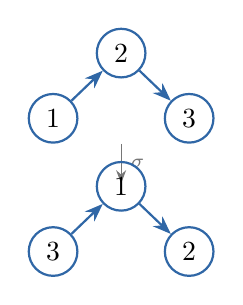
\begin{tikzpicture}[>=Stealth,scale=0.72]
        \node[circle,draw=diagramblue,thick,minimum size=6mm] (a1) at (0,1.9) {$1$};
        \node[circle,draw=diagramblue,thick,minimum size=6mm] (a2) at (1.2,3.05) {$2$};
        \node[circle,draw=diagramblue,thick,minimum size=6mm] (a3) at (2.4,1.9) {$3$};
        \draw[->,thick,diagramblue] (a1)--(a2);
        \draw[->,thick,diagramblue] (a2)--(a3);
        \draw[->,softgray] (1.2,1.45)--node[right,font=\scriptsize] {$\sigma$}(1.2,0.75);
        \node[circle,draw=diagramblue,thick,minimum size=6mm] (b1) at (0,-0.45) {$3$};
        \node[circle,draw=diagramblue,thick,minimum size=6mm] (b2) at (1.2,0.70) {$1$};
        \node[circle,draw=diagramblue,thick,minimum size=6mm] (b3) at (2.4,-0.45) {$2$};
        \draw[->,thick,diagramblue] (b1)--(b2);
        \draw[->,thick,diagramblue] (b2)--(b3);
      \end{tikzpicture}

      \vspace{0.55cm}
      \raggedright
      Labels change; the motif type does not. This is the natural level for macroscopic network statistics.
    \end{column}
  \end{columns}
\end{frame}

%%%%%%%%%%%%%%%%%%%%%%%%%%%%%%%%%%%%%%%%%%%%%%%%%%%%%%%%%%%%%%%%%%%%%%%%%%%%%%%%%%%%%%%%%%%%%%%%%%%%%%%%%%%%%%%%%%%%%%%%
\section{Stochastic Dynamics}

% 8
\begin{frame}{Random Graph Processes}
  \small
  \eyebrow{A stochastic trajectory on a finite graph space}

  A random graph process is a family
  \[
    X_t:\Omega\longrightarrow\mathcal G_N,
    \qquad
    \mu_t(G)=\mathbb P(X_t=G).
  \]

  \begin{center}
  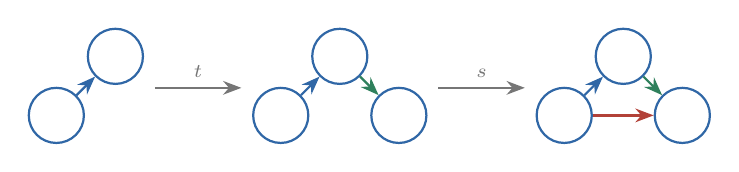
\begin{tikzpicture}[>=Stealth,thick]
    \node[circle,draw=diagramblue,minimum size=7mm] (g0a) at (0,0) {};
    \node[circle,draw=diagramblue,minimum size=7mm] (g0b) at (0.75,0.75) {};
    \draw[->,diagramblue] (g0a)--(g0b);
    \draw[->,softgray] (1.25,0.35)--node[above,font=\scriptsize] {$t$}(2.35,0.35);
    \node[circle,draw=diagramblue,minimum size=7mm] (g1a) at (2.85,0) {};
    \node[circle,draw=diagramblue,minimum size=7mm] (g1b) at (3.60,0.75) {};
    \node[circle,draw=diagramblue,minimum size=7mm] (g1c) at (4.35,0) {};
    \draw[->,diagramblue] (g1a)--(g1b);
    \draw[->,diagramgreen] (g1b)--(g1c);
    \draw[->,softgray] (4.85,0.35)--node[above,font=\scriptsize] {$s$}(5.95,0.35);
    \node[circle,draw=diagramblue,minimum size=7mm] (g2a) at (6.45,0) {};
    \node[circle,draw=diagramblue,minimum size=7mm] (g2b) at (7.20,0.75) {};
    \node[circle,draw=diagramblue,minimum size=7mm] (g2c) at (7.95,0) {};
    \draw[->,diagramblue] (g2a)--(g2b);
    \draw[->,diagramgreen] (g2b)--(g2c);
    \draw[->,diagramred] (g2a)--(g2c);
  \end{tikzpicture}
  \end{center}

  The Markov property is encoded by transition probabilities
  \[
    P_t(H\mid G)=\mathbb P(X_t=H\mid X_0=G),
  \]
  satisfying the Chapman--Kolmogorov identity
  \[
    P_{t+s}(K\mid G)=\sum_{H\in\mathcal G_N}
    P_s(K\mid H)P_t(H\mid G).
  \]
\end{frame}

% 9
\begin{frame}{Forward and Backward Markov Semigroups}
  \small
  \begin{columns}[T,onlytextwidth]
    \begin{column}{0.46\textwidth}
      \eyebrow{Distributions move forward}
      \[
        (T_t^*\mu)(H)
        =\sum_{G\in\mathcal G_N}P_t(H\mid G)\mu(G).
      \]
      If $\mu_0$ is the initial law, then
      \[
        \mu_t=T_t^*\mu_0.
      \]
      The operator $T_t^*$ transports probability mass across graph states.
    \end{column}
    \begin{column}{0.04\textwidth}
      \centering
      {\color{lightgray}\rule{0.45pt}{5.4cm}}
    \end{column}
    \begin{column}{0.46\textwidth}
      \eyebrow{Observables move backward}
      \begin{align*}
        (T_tf)(G)
        &=\sum_{H\in\mathcal G_N}P_t(H\mid G)f(H)\\
        &=\mathbb E[f(X_t)\mid X_0=G].
      \end{align*}
      The two descriptions are dual:
      \[
        \langle T_t^*\mu,f\rangle
        =\langle\mu,T_tf\rangle.
      \]
      Both satisfy $T_{t+s}=T_tT_s$.
    \end{column}
  \end{columns}
\end{frame}

% 10
\begin{frame}{Transition Rates and the Infinitesimal Generator}
  \small
  \eyebrow{Local transition rules determine global evolution}

  Let $W(G\to H)$ be the instantaneous rate of a jump from $G$ to $H$.
  The generator of the backward semigroup is
  \[
    \mathcal Lf
    =\lim_{h\downarrow0}\frac{T_hf-f}{h}.
  \]
  On the finite graph state space,
  \[
    (\mathcal Lf)(G)
    =\sum_{H\neq G}W(G\to H)\,[f(H)-f(G)].
  \]

  \vspace{0.30cm}
  \begin{columns}[T,onlytextwidth]
    \begin{column}{0.47\textwidth}
      \keyterm{Conservation}\par
      Constants do not evolve: $\mathcal L\mathbf 1=0$.
    \end{column}
    \begin{column}{0.47\textwidth}
      \keyterm{Semigroup reconstruction}\par
      In finite dimension, $T_t=e^{t\mathcal L}$.
    \end{column}
  \end{columns}

  \vspace{0.35cm}
  {\color{softgray}\small
  The generator is the bridge from microscopic update mechanisms to equations for network observables.}
\end{frame}

% 11
\begin{frame}{Master Equation and Observable Dynamics}
  \small
  \begin{columns}[T,onlytextwidth]
    \begin{column}{0.66\textwidth}
      \eyebrow{Forward equation for probability}
      \begin{align*}
        \frac{\dd}{\dd t}\mu_t(G)
        ={}&\sum_{H\neq G}W(H\to G)\mu_t(H)\\
        &-\mu_t(G)\sum_{H\neq G}W(G\to H).
      \end{align*}
      The first term is probability gain; the second is probability loss.

      \vspace{0.45cm}
      \eyebrow{Backward equation for observables}
      \[
        \frac{\dd}{\dd t}\langle f\rangle_t
        =\langle\mathcal Lf\rangle_t
        =\langle\mathcal L^*\mu_t,f\rangle.
      \]
    \end{column}
    \begin{column}{0.29\textwidth}
      \centering
      \vspace{0.65cm}
      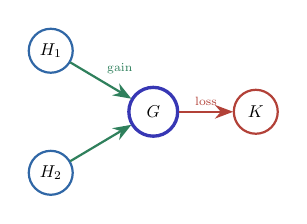
\begin{tikzpicture}[>=Stealth,thick,scale=0.62,transform shape]
        \node[circle,draw=diagramblue,minimum size=9mm] (h1) at (0,1.25) {$H_1$};
        \node[circle,draw=diagramblue,minimum size=9mm] (h2) at (0,-1.25) {$H_2$};
        \node[circle,draw=accent,very thick,minimum size=10mm] (g) at (2.1,0) {$G$};
        \node[circle,draw=diagramred,minimum size=9mm] (k) at (4.2,0) {$K$};
        \draw[->,diagramgreen] (h1)--node[above right,font=\scriptsize] {gain}(g);
        \draw[->,diagramgreen] (h2)--(g);
        \draw[->,diagramred] (g)--node[above,font=\scriptsize] {loss}(k);
      \end{tikzpicture}
    \end{column}
  \end{columns}
\end{frame}

% 12
\begin{frame}{Symmetry Reduction and Observable Hierarchies}
  \small
  \eyebrow{When dynamics respects vertex relabeling}

  If the rates satisfy
  \[
    W(\sigma G\to\sigma H)=W(G\to H),
  \]
  then the generator is equivariant:
  \[
    \mathcal L(\sigma\!\cdot\!f)
    =\sigma\!\cdot\!(\mathcal Lf),
    \qquad
    \mathcal L\mathcal A_N^{S_N}\subseteq\mathcal A_N^{S_N}.
  \]

  \begin{center}
  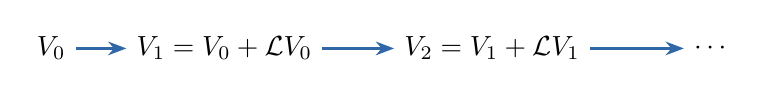
\begin{tikzpicture}[>=Stealth,thick]
    \node (v0) at (0,0) {$V_0$};
    \node (v1) at (2.2,0) {$V_1=V_0+\mathcal LV_0$};
    \node (v2) at (5.6,0) {$V_2=V_1+\mathcal LV_1$};
    \node (vd) at (8.4,0) {$\cdots$};
    \draw[->,diagramblue] (v0)--(v1);
    \draw[->,diagramblue] (v1)--(v2);
    \draw[->,diagramblue] (v2)--(vd);
  \end{tikzpicture}
  \end{center}

  Starting from chosen observables, repeatedly apply $\mathcal L$ until the generated subspace closes. Exact low-dimensional dynamics exists when
  \[
    \mathcal LV_k\subseteq V_k.
  \]
\end{frame}

%%%%%%%%%%%%%%%%%%%%%%%%%%%%%%%%%%%%%%%%%%%%%%%%%%%%%%%%%%%%%%%%%%%%%%%%%%%%%%%%%%%%%%%%%%%%%%%%%%%%%%%%%%%%%%%%%%%%%%%%
\section{ Model}

% 13
\begin{frame}{Example Model: Three Microscopic Mechanisms}
  \small
  \eyebrow{Single-edge transitions for a directed network}

  \begin{columns}[T,onlytextwidth]
    \begin{column}{0.31\textwidth}
      \centering
      {\color{diagramblue}\bfseries Spontaneous creation}\par
      \vspace{0.18cm}
      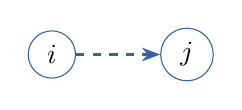
\begin{tikzpicture}[>=Stealth,scale=0.78]
        \node[circle,draw=diagramblue,minimum size=6mm] (i) at (0,0) {$i$};
        \node[circle,draw=diagramblue,minimum size=6mm] (j) at (2.2,0) {$j$};
        \draw[->,dashed,diagramblue,thick] (i)--(j);
      \end{tikzpicture}
      \[
        r_{ij}^{(\alpha)}=(1-x_{ij})\frac{\alpha}{N}.
      \]
      A missing edge appears at a homogeneous baseline rate.
    \end{column}
    \begin{column}{0.31\textwidth}
      \centering
      {\color{diagramred}\bfseries Deletion}\par
      \vspace{0.18cm}
      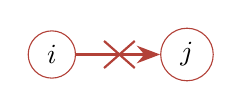
\begin{tikzpicture}[>=Stealth,scale=0.78]
        \node[circle,draw=diagramred,minimum size=6mm] (i) at (0,0) {$i$};
        \node[circle,draw=diagramred,minimum size=6mm] (j) at (2.2,0) {$j$};
        \draw[->,diagramred,very thick] (i)--(j);
        \draw[diagramred,thick] (0.85,-0.22)--(1.35,0.22);
        \draw[diagramred,thick] (0.85,0.22)--(1.35,-0.22);
      \end{tikzpicture}
      \[
        r_{ij}^{(\gamma)}=\gamma x_{ij}.
      \]
      An existing edge disappears independently of other edges.
    \end{column}
    \begin{column}{0.31\textwidth}
      \centering
      {\color{diagramgreen}\bfseries Two-path closure}\par
      \vspace{0.18cm}
      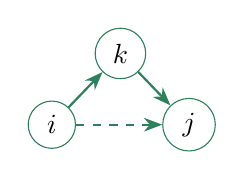
\begin{tikzpicture}[>=Stealth,scale=0.67]
        \node[circle,draw=diagramgreen,minimum size=6mm] (i) at (0,0) {$i$};
        \node[circle,draw=diagramgreen,minimum size=6mm] (k) at (1.3,1.35) {$k$};
        \node[circle,draw=diagramgreen,minimum size=6mm] (j) at (2.6,0) {$j$};
        \draw[->,diagramgreen,thick] (i)--(k);
        \draw[->,diagramgreen,thick] (k)--(j);
        \draw[->,dashed,diagramgreen,thick] (i)--(j);
      \end{tikzpicture}
      \[
        \begin{aligned}
        r_{ij}^{(\beta)}={}&\beta(1-x_{ij})\\[-2pt]
        &\times\!\sum_{k\neq i,j}x_{ik}x_{kj}.
        \end{aligned}
      \]
      Open directed two-paths promote transitive closure.
    \end{column}
  \end{columns}
\end{frame}

% 14
\begin{frame}{Generator Acting on a Single Edge}
  \small
  \eyebrow{Microscopic rule translated into algebra}

  Combining creation and closure gives the addition rate
  \[
    r_{ij}^{+}=(1-x_{ij})
    \left[\frac{\alpha}{N}+\beta\sum_{k\neq i,j}x_{ik}x_{kj}\right],
    \qquad
    r_{ij}^{-}=\gamma x_{ij}.
  \]
  Since an update of edge $(i,j)$ changes $x_{ij}$ by $+1$ or $-1$,
  \[
    \mathcal Lx_{ij}
    =(1-x_{ij})
    \left[\frac{\alpha}{N}+\beta\sum_{k\neq i,j}x_{ik}x_{kj}\right]
    -\gamma x_{ij}.
  \]

  \vspace{0.25cm}
  Taking expectations yields
  \begin{align*}
    \frac{\dd}{\dd t}\langle x_{ij}\rangle
    ={}&\frac{\alpha}{N}
    -\left(\frac{\alpha}{N}+\gamma\right)\langle x_{ij}\rangle\\
    &+\beta\sum_{k\neq i,j}
    \left(\langle x_{ik}x_{kj}\rangle
    -\langle x_{ij}x_{ik}x_{kj}\rangle\right).
  \end{align*}
\end{frame}

% 15
\begin{frame}{Edge Count, Open Two-Paths, and the Closure Problem}
  \small
  \begin{columns}[T,onlytextwidth]
    \begin{column}{0.66\textwidth}
      \eyebrow{Two structural observables}
      \[
        M=\sum_{i\neq j}x_{ij},
        \qquad
        Q=\sum_{i\neq j}\sum_{k\neq i,j}
        (1-x_{ij})x_{ik}x_{kj}.
      \]
      Their first evolution equation is
      \[
        \frac{\dd}{\dd t}\langle M\rangle
        =\frac{\alpha}{N}\big[N(N-1)-\langle M\rangle\big]
        -\gamma\langle M\rangle+\beta\langle Q\rangle.
      \]
      When $\beta=0$, the edge count closes exactly. When $\beta\neq0$, two-path closure couples $M$ to $Q$, and $Q$ generally couples to higher-order motifs.
    \end{column}
    \begin{column}{0.29\textwidth}
      \centering
      \vspace{0.55cm}
      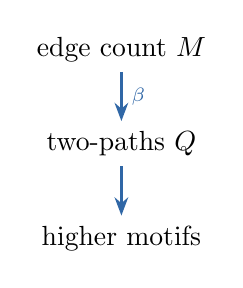
\begin{tikzpicture}[>=Stealth,thick]
        \node (m) at (0,1.8) {edge count $M$};
        \node (q) at (0,0.6) {two-paths $Q$};
        \node (h) at (0,-0.6) {higher motifs};
        \draw[->,diagramblue] (m)--node[right,font=\scriptsize] {$\beta$}(q);
        \draw[->,diagramblue] (q)--(h);
      \end{tikzpicture}

      \vspace{0.55cm}
      \raggedright
      \keyterm{Central question}\par
      Which invariant observable space is closed under $\mathcal L$, exactly or approximately?
    \end{column}
  \end{columns}

  \vfill
  {\color{softgray}\small
  Algebra identifies the hierarchy; stochastic dynamics determines how information propagates through it.}
\end{frame}

\end{document}
